\chapter{От квантов открытой струны к тахионам и гравитации}

\lectureoverview{Теперь мы квантуем нормальные моды, найденные в предыдущей лекции, и спрашиваем, какие состояния частиц они порождают. Каждая поперечная мода представляет собой гармонический осциллятор, но ее нормировка слегка непривычна: возбуждение моды \(n\) повышает светофронтовую энергию и, следовательно, уровень по квадрату массы на \(n\) единиц. Первый возбужденный уровень открытой струны преобразуется в точности как две поперечные поляризации безмассового вектора. Поэтому релятивистская согласованность фиксирует квадрат массы основного состояния как отрицательный. Это состояние и есть тахион бозонной струны; его истинный смысл состоит в неустойчивости вакуума, а не в том, что это некая практическая сверхсветовая частица. Наконец, как только струны начинают взаимодействовать, слияние и расщепление делают замкнутые струны неизбежными; низшее возбуждение замкнутой струны будет гравитоном.}

\section{Осциллятор, скрытый в каждой моде струны}

Для одной поперечной координаты \(X\) ненулевая нормальная мода с номером \(n\) имеет энергию и лагранжиан

\begin{align}
  E_n
  &=
  \frac14\dot X_n^{\,2}
  +\frac{n^2}{4}X_n^2,
  \label{eq:l03-mode-energy}\\
  L_n
  &=
  \frac14\dot X_n^{\,2}
  -\frac{n^2}{4}X_n^2.
  \label{eq:l03-mode-lagrangian}
\end{align}

Множители \(1/4\) — не ошибка. Они отражают нормировку, выбранную при сведении действия струны к независимым фурье-модам. Поэтому первым шагом при построении гамильтониана является вычисление канонического импульса,

\begin{equation}
  p_n=\frac{\partial L_n}{\partial\dot X_n}
     =\frac12\dot X_n,
  \qquad
  \dot X_n=2p_n.
  \label{eq:l03-canonical-momentum}
\end{equation}

Преобразование Лежандра дает

\begin{equation}
  H_n=p_n\dot X_n-L_n
     =p_n^2+\frac{n^2}{4}X_n^2.
  \label{eq:l03-mode-hamiltonian}
\end{equation}

\begin{figure}[H]
  \centering
  \includegraphics[width=0.82\textwidth]{lecture_03_figure_01.png}
  \caption{Энергия моды, лагранжиан, канонический импульс и гамильтониан в нормировке, унаследованной от открытой струны.}
  \lectureframe{00:05:40}
  \label{fig:l03-mode-hamiltonian-board}
\end{figure}

Чтобы факторизовать \(H_n\), объединим \(X_n\) и \(p_n\) следующим образом:

\begin{equation}
  \frac{nX_n}{2}\pm i p_n.
\end{equation}

Классически эти два множителя коммутировали бы, но квантово-механически

\begin{equation}
  [X_n,p_m]=i\delta_{nm}
  \label{eq:l03-canonical-commutator}
\end{equation}

в единицах, где \(\hbar=1\). Перекрестные члены не сокращаются так уж безобидно. Для фиксированной моды,

\begin{align}
  \left[\frac{nX_n}{2}+ip_n,
        \frac{nX_n}{2}-ip_n\right]
  &=n,
  \label{eq:l03-unscaled-commutator}\\
  \left(\frac{nX_n}{2}-ip_n\right)
  \left(\frac{nX_n}{2}+ip_n\right)
  &=H_n-\frac n2.
  \label{eq:l03-factorized-hamiltonian}
\end{align}

\begin{figure}[H]
  \centering
  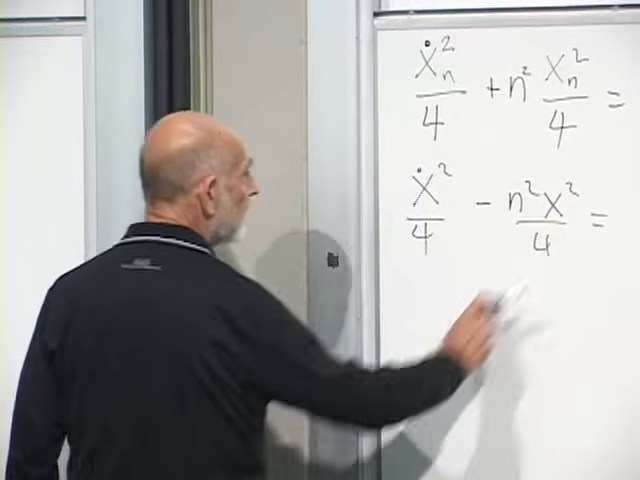
\includegraphics[width=0.82\textwidth]{lecture_03_figure_02.png}
  \caption{Вычисление на доске, в котором канонический коммутатор дает множитель \(n\).}
  \lectureframe{00:10:30}
  \label{fig:l03-commutator-board}
\end{figure}

Множитель \(n\) показывает, как следует нормировать операторы рождения и уничтожения:

\begin{align}
  a_n
  &\equiv
  \frac{\sqrt n}{2}X_n+\frac{i}{\sqrt n}p_n,
  \label{eq:l03-annihilator}\\
  a_n^\dagger
  &\equiv
  \frac{\sqrt n}{2}X_n-\frac{i}{\sqrt n}p_n.
  \label{eq:l03-creator}
\end{align}

Они удовлетворяют соотношениям

\begin{equation}
  [a_n,a_m^\dagger]=\delta_{nm},
  \qquad
  H_n=n\left(a_n^\dagger a_n+\frac12\right).
  \label{eq:l03-oscillator-algebra}
\end{equation}

Таким образом, \(a_n^\dagger\) добавляет один квант \(n\)-го осциллятора, но этот квант несет \(n\) единиц энергии моды. Привычное расстояние между уровнями осциллятора не исчезает; его частота равна \(\omega_n=n\).

\begin{figure}[H]
  \centering
  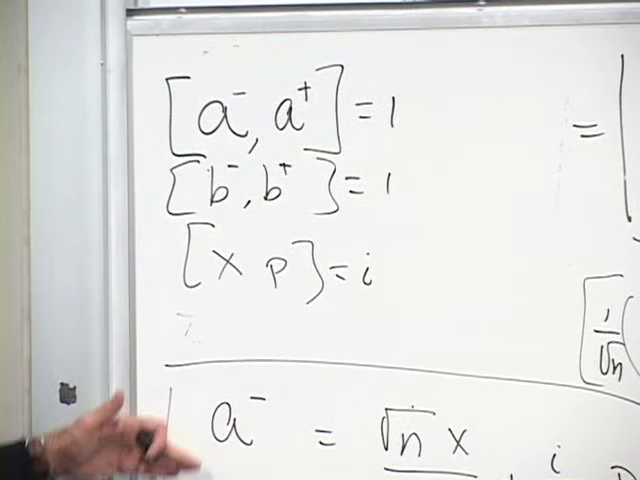
\includegraphics[width=0.82\textwidth]{lecture_03_figure_03.png}
  \caption{Нормированные операторы уничтожения и рождения для \(n\)-го струнного осциллятора.}
  \lectureframe{00:12:00}
  \label{fig:l03-ladder-board}
\end{figure}

\subsection{Две поперечные башни}

В четырех измерениях пространства-времени струна, несущая очень большой импульс вдоль оси \(z\), имеет две поперечные координаты, \(X\) и \(Y\). Поэтому нам нужны две независимые башни осцилляторов. Пусть \(a_n,a_n^\dagger\) действуют на моды \(X\), а \(b_n,b_n^\dagger\) — на моды \(Y\). Решая \eqref{eq:l03-annihilator}--\eqref{eq:l03-creator} относительно координат, получаем

\begin{equation}
  X_n=\frac{a_n+a_n^\dagger}{\sqrt n},
  \qquad
  Y_n=\frac{b_n+b_n^\dagger}{\sqrt n}.
  \label{eq:l03-mode-coordinates}
\end{equation}

\begin{figure}[H]
  \centering
  \includegraphics[width=0.78\textwidth]{lecture_03_figure_04.png}
  \caption{Выражение координаты моды через ее операторы рождения и уничтожения.}
  \lectureframe{00:17:05}
  \label{fig:l03-coordinate-operator-board}
\end{figure}

Координаты открытой струны были разложены по модам Неймана,

\begin{align}
  X(\sigma,\tau)
  &=X_{\rm cm}(\tau)
    +\sum_{n=1}^{\infty}X_n(\tau)\cos(n\sigma),
  \label{eq:l03-X-fourier}\\
  Y(\sigma,\tau)
  &=Y_{\rm cm}(\tau)
    +\sum_{n=1}^{\infty}Y_n(\tau)\cos(n\sigma).
  \label{eq:l03-Y-fourier}
\end{align}

Косинусы появляются потому, что наклоны на концах обращаются в нуль. Подстановка \eqref{eq:l03-mode-coordinates} превращает саму струну в оператор:

\begin{align}
  X(\sigma,\tau)
  &=X_{\rm cm}(\tau)
    +\sum_{n=1}^{\infty}
      \frac{a_n(\tau)+a_n^\dagger(\tau)}{\sqrt n}
      \cos(n\sigma),
  \label{eq:l03-X-operator}\\
  Y(\sigma,\tau)
  &=Y_{\rm cm}(\tau)
    +\sum_{n=1}^{\infty}
      \frac{b_n(\tau)+b_n^\dagger(\tau)}{\sqrt n}
      \cos(n\sigma).
  \label{eq:l03-Y-operator}
\end{align}

\begin{figure}[H]
  \centering
  \begin{minipage}[t]{0.48\textwidth}
    \centering
    \includegraphics[width=\textwidth]{lecture_03_figure_05.png}
    \par\smallskip\footnotesize (a) Разложения координат по модам.
  \end{minipage}\hfill
  \begin{minipage}[t]{0.48\textwidth}
    \centering
    \includegraphics[width=\textwidth]{lecture_03_figure_06.png}
    \par\smallskip\footnotesize (b) Операторы рождения и уничтожения, подставленные в координаты
    струны.
  \end{minipage}
  \caption{Форма квантовой открытой струны собирается из всех ее поперечных операторов осцилляторов.}
  \lectureframe{00:20:35 and 00:21:05}
  \label{fig:l03-string-coordinate-board}
\end{figure}

\begin{classroomqa}
\audiencequestion{Является ли \(X_n\) также функцией \(\sigma\)?\lecturetimestamp{00:21:48}}
\lecturerresponse{Нет. Зависимость от \(\sigma\) целиком содержится в \(\cos(n\sigma)\). Коэффициент \(X_n\) — это зависящая от времени амплитуда этого пространственного профиля, так что \(X_n=X_n(\tau)\).}
\end{classroomqa}

\begin{classroomqa}
\audiencequestion{Почему у операторов, называемых повышающим и понижающим, знаки как будто переставлены местами?\lecturetimestamp{00:23:13}}
\lecturerresponse{Видимый знак \(ip_n\) не является правилом именования. Вычислите коммутатор с гамильтонианом. Оператор, удовлетворяющий \([H_n,a_n^\dagger]=n a_n^\dagger\), повышает энергию; удовлетворяющий \([H_n,a_n]=-n a_n\), понижает ее.}
\end{classroomqa}

Две поперечные башни — это наглядная четырехмерная картина. Согласованно квантуемая бозонная струна имеет 26 измерений пространства-времени, так что у нее 24 семейства поперечных осцилляторов, а не 2. Логика ниже не меняется: число состояний первого уровня должно совпадать с числом физических поляризаций безмассового вектора в той же размерности.

\section{Массивный спин и безмассовый гелицитет}

Прежде чем приписывать спин струнным состояниям, нужно провести одно четкое различие. Массивная частица со спином \(J\) имеет \(2J+1\) спиновых состояний,

\begin{equation}
  m_J=-J,-J+1,\ldots,J-1,J.
  \label{eq:l03-massive-spin-multiplet}
\end{equation}

Например, массивная частица со спином 1 имеет 3 поляризации, а массивная частица со спином 2 — 5. Понять почему можно, перейдя в систему покоя. Там доступны все пространственные вращения. Поверните ось спина, затем выполните обратный буст, и окажется, что все \(2J+1\) компонент относятся к одной и той же релятивистской частице.

У безмассовой частицы нет системы покоя. Ее инвариантная спиновая метка — это гелицитет, то есть момент импульса вдоль направления ее движения. У фотона есть только \(h=+1\) и \(h=-1\); у гравитона — только \(h=+2\) и \(h=-2\). Скаляр имеет одно состояние с \(h=0\). В лекции для спаривания двух гелицитетов используется симметрия отражения. В хиральной теории одно безмассовое неприводимое представление может нести только один гелицитет, так что такое спаривание является дополнительным утверждением о симметрии, а не следствием одной лишь безмассовости.\editorialnote{Современная классификация по маленькой группе допускает безмассовые представления с одним гелицитетом. Четность или подходящее CPT-полное содержание полей обеспечивает противоположный гелицитет в привычных примерах фотона и гравитона.}

\begin{figure}[H]
  \centering
  \begin{minipage}[t]{0.45\textwidth}
    \centering
    \includegraphics[width=\textwidth]{lecture_03_figure_07.png}
    \par\smallskip\footnotesize (a) Подсчет спиновых состояний, начатый на доске.
  \end{minipage}\hfill
  \begin{minipage}[t]{0.5\textwidth}
    \centering
    \begin{adjustbox}{max width=\linewidth}
    \begin{tabular}{@{}ccc@{}}
      \toprule
      Спин & Массивные состояния & Безмассовые гелицитеты \\
      \midrule
      \(0\) & \(1\) & \(0\) \\
      \(1\) & \(3\) & \(+1,-1\) \\
      \(2\) & \(5\) & \(+2,-2\) \\
      \bottomrule
    \end{tabular}
    \end{adjustbox}
  \end{minipage}
  \caption{Масса устраняет систему покоя, а вместе с ней и промежуточные проекции спина.}
  \lectureframe{00:27:40}
  \label{fig:l03-spin-count}
\end{figure}

\subsection{Линейная и круговая поляризация фотона}

Рассмотрим фотон, движущийся вдоль \(z\). Его две поперечные линейные поляризации — \(\ket{x}\) и \(\ket{y}\). Они не являются собственными состояниями гелицитета. Круговые состояния имеют вид

\begin{align}
  \ket{R}
  &=\frac{1}{\sqrt2}\left(\ket{x}+i\ket{y}\right),
  \label{eq:l03-right-circular}\\
  \ket{L}
  &=\frac{1}{\sqrt2}\left(\ket{x}-i\ket{y}\right),
  \label{eq:l03-left-circular}
\end{align}

с гелицитетами \(+1\) и \(-1\), с точностью до соглашения о том, что называть правым и левым. Линейно поляризованный фотон является суперпозицией этих двух исходов. Его средний гелицитет может обращаться в нуль, но измерение гелицитета никогда не обнаруживает фотон со спином 0. Аналогично,

\begin{equation}
  \frac{1}{\sqrt2}\left(\ket{x}+\ket{y}\right)
\end{equation}

Это просто линейная поляризация под углом 45 градусов.

\begin{figure}[H]
  \centering
  \begin{minipage}[t]{0.48\textwidth}
    \centering
    \includegraphics[width=\textwidth]{lecture_03_figure_08.png}
    \par\smallskip\footnotesize (a) Состояния круговой поляризации на доске.
  \end{minipage}\hfill
  \begin{minipage}[t]{0.48\textwidth}
    \centering
    \begin{adjustbox}{max width=\linewidth}
    \begin{tikzpicture}[>=Latex,scale=0.9]
      \draw[->,thick] (0,0) -- (3.4,0) node[right] {\(z\)};
      \draw[->,blue!70!black,thick] (0,0) -- (0,2.0)
        node[above] {\(x\)};
      \draw[->,orange!85!black,thick] (0,0) -- (-1.4,-1.2)
        node[below left] {\(y\)};
      \draw[red!70!black,thick,->]
        plot[domain=0:320,samples=80]
        ({1.0*cos(\x)},{0.58*sin(\x)+0.4});
      \node[red!70!black] at (1.55,1.25) {circular};
    \end{tikzpicture}
    \end{adjustbox}
  \end{minipage}
  \caption{Линейная поляризация задает поперечный базис; круговые комбинации диагонализуют гелицитет.}
  \lectureframe{00:37:45}
  \label{fig:l03-polarization}
\end{figure}

\begin{classroomqa}
\audiencequestion{Похоже ли это на разделение спиновых состояний в эксперименте Штерна--Герлаха?\lecturetimestamp{00:37:40}}
\lecturerresponse{Идея квантовой суперпозиции та же, но для фотона естественнее говорить о поляризации. Измерение круговой поляризации различает два гелицитета; в пучке нет продольного фотона со спином 0.}
\end{classroomqa}

Гравитон повторяет ту же схему при спине 2. Для учета спина можно схематически записать

\begin{equation}
  \ket{+2}\sim\ket{+1}\otimes\ket{+1},
  \qquad
  \ket{-2}\sim\ket{-1}\otimes\ket{-1}.
  \label{eq:l03-graviton-helicity}
\end{equation}

Это не означает, что гравитон буквально состоит из двух фотонов. Это означает, что две одинаковые спиральности складываются в правильную спиральность частицы со спином 2.

\begin{classroomqa}
\audiencequestion{Распространяется ли аналогия с двумя фотонами на другие квантовые числа?\lecturetimestamp{00:41:05}}
\lecturerresponse{Нет, если понимать её как составную модель. Существуют мощные формулы, в которых гравитационные амплитуды выглядят как произведения или ``квадраты'' амплитуд калибровочной теории, однако гравитон всё равно остаётся самостоятельной частицей. Здесь эта аналогия наиболее надёжна как утверждение о спиральности.\editorialnote{Современные соотношения Kawai--Lewellen--Tye и double-copy делают утверждение об амплитудах точным в подходящих теориях; они не превращают гравитон в связанное состояние двух фотонов.}}
\end{classroomqa}

\begin{classroomqa}
\audiencequestion{Фотон может иметь любой импульс; не следует ли тогда, что у него непрерывный, а не изолированный спектр, как требуется для частицы?\lecturetimestamp{00:42:17}}
\lecturerresponse{Непрерывной переменной является импульс центра масс. Зафиксируйте этот импульс и посмотрите на внутреннюю инвариантную массу. Частица определяется изолированным массовым уровнем; изменение её полного импульса затем порождает обычное непрерывное дисперсионное соотношение.}
\end{classroomqa}

\section{Низшие уровни открытой струны}

Теперь мы можем вернуться к струне. В описании при большом импульсе конечная внутренняя энергия на световом фронте пропорциональна квадрату инвариантной массы. Опуская общий струнный масштаб, запишем спектр в виде

\begin{equation}
  \begin{aligned}
    M^2
    &=m_0^2
      +\sum_{n=1}^{\infty}n
       \left(N_n^{(a)}+N_n^{(b)}\right),\\
    N_n^{(a)}&=a_n^\dagger a_n,
    \qquad
    N_n^{(b)}=b_n^\dagger b_n.
  \end{aligned}
  \label{eq:l03-open-spectrum}
\end{equation}

Основное состояние осциллятора удовлетворяет

\begin{equation}
  a_n\ket{0}=0,
  \qquad
  b_n\ket{0}=0,
  \qquad n=1,2,\ldots .
  \label{eq:l03-ground-annihilation}
\end{equation}

Это не пустое отсутствие струны. Это квантовая струна с наименьшим возбуждением, и её координаты всё ещё флуктуируют. Обозначим её квадрат массы через \(m_0^2\); он пока не определён.

\begin{figure}[H]
  \centering
  \includegraphics[width=0.78\textwidth]{lecture_03_figure_09.png}
  \caption{Основное состояние открытой струны и определяющие его условия аннигиляции.}
  \lectureframe{00:45:20}
  \label{fig:l03-ground-state-board}
\end{figure}

Простейшие возбуждения получаются действием операторов рождения \(n=1\):

\begin{equation}
  a_1^\dagger\ket{0},
  \qquad
  b_1^\dagger\ket{0},
  \qquad
  M^2=m_0^2+1.
  \label{eq:l03-first-level}
\end{equation}

\begin{figure}[H]
  \centering
  \includegraphics[width=0.78\textwidth]{lecture_03_figure_10.png}
  \caption{Одно из двух вырожденных состояний первого уровня; приращение его квадрата массы записано на доске.}
  \lectureframe{00:49:25}
  \label{fig:l03-first-level-board}
\end{figure}

``единица'' в eqref{eq:l03-first-level} — это не один джоуль, не один электрон-вольт и не одна масса Планка. Мы опустили размерный струнный масштаб. Пока она означает одну ступень на лестнице значений квадрата массы осциллятора; недостающие единицы будут восстановлены на следующей лекции.

Любая линейная комбинация двух вырожденных состояний также является состоянием этого уровня. В частности,

\begin{equation}
  \frac{1}{\sqrt2}
  \left(a_1^\dagger\pm i b_1^\dagger\right)\ket{0}
  \label{eq:l03-string-circular-states}
\end{equation}

является струнным аналогом круговой поляризации. При повороте в плоскости \(x\)-\(y\) \(a_1^\dagger\) и \(b_1^\dagger\) преобразуются как две компоненты поперечного вектора. Поэтому комбинации в \eqref{eq:l03-string-circular-states} имеют спиральность \(+1\) и \(-1\).

\begin{figure}[H]
  \centering
  \includegraphics[width=0.82\textwidth]{lecture_03_figure_11.png}
  \caption{На доске собраны условия для основного состояния, два возбуждения первого уровня и их круговые комбинации.}
  \lectureframe{00:56:00}
  \label{fig:l03-level-structure-board}
\end{figure}

Третьего вырожденного состояния, которое могло бы играть роль продольной поляризации, нет. Если бы эти два состояния имели ненулевую массу, релятивистской частице со спином 1 потребовались бы три поляризации. При ровно двух поляризациях состояние должно быть безмассовым. Следовательно,

\begin{equation}
  m_0^2+1=0,
  \qquad
  m_0^2=-1.
  \label{eq:l03-intercept-condition}
\end{equation}

Первый уровень фотоноподобен: это безмассовое калибровочное векторное состояние. Это не обязательно фотон электромагнетизма; то, какой калибровочной частице оно в итоге соответствует, зависит от модели струны. Лежащее ниже него основное состояние имеет отрицательный квадрат массы. Это тахион бозонной открытой струны.\editorialnote{В полной критической бозонной струне интерсепт при нормальном упорядочении и алгебра Лоренца связаны с \(D=26\). Вычисление в лекции с двумя поперечными направлениями — это четырёхмерная тень того же аргумента подсчёта состояний: \(D-2\) осцилляторных состояний первого уровня соответствуют \(D-2\) физическим поляризациям безмассового вектора.}

\begin{classroomqa}
\audiencequestion{Почему нас должно волновать, что \(m_0^2\) отрицательно?\lecturetimestamp{00:56:35}}
\lecturerresponse{Потому что квадрат массы — это кривизна квадратичного потенциала поля вблизи состояния, которое мы назвали вакуумом. Отрицательная кривизна означает, что эта конфигурация не является устойчивым основным состоянием. Следующее вычисление делает это утверждение точным.}
\end{classroomqa}

\section{Что на самом деле означает тахион}

Само название ``тахион'' подталкивает к вводящей в заблуждение первой мысли. Начнём с релятивистского дисперсионного соотношения при \(c=1\),

\begin{equation}
  E(p)=\sqrt{p^2+m^2}.
  \label{eq:l03-relativistic-dispersion}
\end{equation}

Для волнового пакета групповая скорость равна

\begin{equation}
  v_g=\frac{dE}{dp}.
  \label{eq:l03-group-velocity}
\end{equation}

Это воспроизводит знакомые случаи:

\begin{align}
  E_{\rm nr}(p)&=\frac{p^2}{2m},
  &v_g&=\frac{p}{m},
  \label{eq:l03-nr-group-velocity}\\
  E_\gamma(p)&=|p|,
  &|v_g|&=1,
  \label{eq:l03-photon-group-velocity}\\
  E_m(p)&=\sqrt{p^2+m^2},
  &|v_g|&=\frac{|p|}{\sqrt{p^2+m^2}}<1.
  \label{eq:l03-massive-group-velocity}
\end{align}

\begin{figure}[H]
  \centering
  \begin{minipage}[t]{0.48\textwidth}
    \centering
    \includegraphics[width=\textwidth]{lecture_03_figure_12.png}
    \par\smallskip\footnotesize (a) Нерелятивистская групповая скорость.
  \end{minipage}\hfill
  \begin{minipage}[t]{0.48\textwidth}
    \centering
    \includegraphics[width=\textwidth]{lecture_03_figure_13.png}
    \par\smallskip\footnotesize (b) Релятивистское дисперсионное соотношение и его производная.
  \end{minipage}
  \caption{Скорость распространения считывается по наклону \(E(p)\).}
  \lectureframe{01:01:50 and 01:03:15}
  \label{fig:l03-group-velocity-board}
\end{figure}

Если \(m^2=-\mu^2\), то формальное выражение принимает вид

\begin{equation}
  E(p)=\sqrt{p^2-\mu^2},
  \qquad
  v_g=\frac{p}{\sqrt{p^2-\mu^2}},
  \label{eq:l03-formal-tachyon-dispersion}
\end{equation}

что даёт \(|v_g|>1\), когда квадратный корень веществен. Но это не правильная физическая интерпретация основного состояния бозонной струны. Проблема возникает уже при малом импульсе, где частота мнима.

\subsection{Отрицательная кривизна потенциала поля}

Рассмотрим вещественное скалярное поле в одном пространственном измерении,

\begin{equation}
  \left(\partial_t^2-\partial_x^2+m^2\right)\phi=0.
  \label{eq:l03-klein-gordon}
\end{equation}

Для плоской волны \(\phi\propto e^{-i\omega t+ikx}\),

\begin{equation}
  \omega^2=k^2+m^2.
  \label{eq:l03-kg-dispersion}
\end{equation}

\begin{figure}[H]
  \centering
  \includegraphics[width=0.82\textwidth]{lecture_03_figure_14.png}
  \caption{Уравнение Klein--Gordon, используемое для выявления неустойчивости, скрытой за отрицательным квадратом массы.}
  \lectureframe{01:06:40}
  \label{fig:l03-klein-gordon-board}
\end{figure}

Сохраняющаяся квадратичная энергия имеет вид

\begin{equation}
  \mathcal E
  =\frac12\int dx\,
  \left[
    \dot\phi^{\,2}
    +(\partial_x\phi)^2
    +m^2\phi^2
  \right].
  \label{eq:l03-field-energy}
\end{equation}

\begin{figure}[H]
  \centering
  \includegraphics[width=0.82\textwidth]{lecture_03_figure_15.png}
  \caption{Энергия скалярного поля, где массовый член задаёт локальную кривизну потенциала.}
  \lectureframe{01:08:10}
  \label{fig:l03-field-energy-board}
\end{figure}

При \(m^2>0\) локальный потенциал \(V(\phi)=\tfrac12m^2\phi^2\) представляет собой чашу. Конфигурация \(\phi=0\) находится на её дне. При \(m^2=-\mu^2\) та же точка является вершиной перевёрнутой чаши. Уравнение \eqref{eq:l03-kg-dispersion} принимает вид

\begin{equation}
  \omega^2=k^2-\mu^2.
  \label{eq:l03-tachyonic-modes}
\end{equation}

Для мод с \(k^2<\mu^2\) имеем

\begin{equation}
  \omega=\pm i\sqrt{\mu^2-k^2},
  \qquad
  \phi_k(t)\propto
  e^{\pm\sqrt{\mu^2-k^2}\,t}.
  \label{eq:l03-growing-mode}
\end{equation}

Одна из ветвей растёт экспоненциально. Следовательно, этот якобы вакуум неустойчив: сколь угодно малое длинноволновое возмущение уводит поле от \(\phi=0\). Именно это и означает тахион в спектре.

\subsection{Цепочка перевёрнутых маятников}

Ряд связанных маятников наглядно показывает это различие. Поставьте каждый маятник вертикально вверх. Однородная конфигурация существует, но она находится в равновесии при максимуме потенциальной энергии. Слегка толкните один маятник — и он упадёт, увлекая за собой соседние. Фронт падения распространяется по цепочке с конечной скоростью сигнала, задаваемой связями.

\begin{figure}[H]
  \centering
  \begin{minipage}[t]{0.48\textwidth}
    \centering
    \includegraphics[width=\textwidth]{lecture_03_figure_16.png}
    \par\smallskip\footnotesize (a) Модель связанных перевёрнутых маятников на доске.
  \end{minipage}\hfill
  \begin{minipage}[t]{0.48\textwidth}
    \centering
    \begin{adjustbox}{max width=\linewidth}
    \begin{tikzpicture}[>=Latex,scale=0.78]
      \draw[thick] (-0.3,0) -- (6.3,0);
      \foreach \x/\a in {0/0,1/0,2/8,3/28,4/55,5/72,6/78}{
        \fill (\x,0) circle (0.06);
        \draw[thick] (\x,0) -- ++({90-\a}:1.25);
        \fill[blue!65!black]
          ($(\x,0)+({90-\a}:1.25)$) circle (0.11);
      }
      \draw[red!70!black,->,thick] (1.7,-0.45) -- (4.6,-0.45)
        node[midway,below] {falling front};
    \end{tikzpicture}
    \end{adjustbox}
  \end{minipage}
  \caption{Фронт падения неустойчивости распространяется по системе причинным образом, хотя её линеаризованный спектр содержит отрицательный квадрат массы.}
  \lectureframe{01:10:40}
  \label{fig:l03-pendulum-instability}
\end{figure}

Ничто в этом механизме не позволяет управляемому сигналу обогнать причинный фронт. Тахионная мода указывает на неудачную точку разложения, а не на устойчивого сверхсветового переносчика.\editorialnote{Для локального релятивистского уравнения поля скорость фронта остаётся причинной скоростью. Формальная групповая скорость вещественной ветви при больших \(k\) не превращает нестабильный вакуум в канал связи быстрее света.}

\begin{classroomqa} \audiencequestion{Является ли только что найденное безмассовое состояние тем самым гравитоном, который предсказывает теория струн?\lecturetimestamp{01:14:27}} \lecturerresponse{Нет. Это состояние открытой струны со спином 1 и двумя поляризациями, так что по своей природе оно подобно калибровочному бозону. Гравитон — это возбуждение замкнутой струны со спином 2.} \end{classroomqa}

\begin{classroomqa} \audiencequestion{Допустим ли математически перевёрнутый потенциал, и где система закончила бы после падения?\lecturetimestamp{01:15:17}} \lecturerresponse{Как локальное приближение он вполне допустим, но сам по себе не имеет основного состояния, потому что энергия не ограничена снизу. Более полный потенциал может затем снова загнуться вверх и иметь более низкий минимум. Тогда система скатывается или конденсируется к этой устойчивой конфигурации.} \end{classroomqa}

Обычная бозонная струна имеет именно этот дефект. Её более высокие осцилляторные состояния остаются частью спектра, но это возбуждения неустойчивого фона. Согласованные теории суперструн устраняют тахион открытой струны в своих устойчивых секторах, сохраняя при этом безмассовые и массивные струнные возбуждения.

\begin{classroomqa} \audiencequestion{Совпадают ли и другие свойства состояния открытой струны с фотоном так же хорошо, как его две поляризации?\lecturetimestamp{01:17:07}} \lecturerresponse{Это состояние ведёт себя как безмассовый калибровочный бозон. Его конкретные зарядовые квантовые числа, правила излучения и то, с чем именно его следует отождествлять, зависят от струнной модели, так что его следует называть фотоноподобным, а не сразу отождествлять с электромагнетизмом. Эти свойства взаимодействия обсуждаются позже.} \end{classroomqa}

\section{Как взаимодействуют струны}

Свободный спектр — лишь половина теории. Струны также соединяются и расщепляются. Сначала полезно вспомнить, что возбуждённая свободная струна может нести угловой момент. Прямая вращающаяся струна вращается вокруг своего центра масс, и её энергия и угловой момент растут вместе вдоль знакомой струнной траектории.

\begin{figure}[H] \centering
  \includegraphics[width=0.72\textwidth]{lecture_03_figure_17.png} \caption{Схема вращающейся открытой струны вокруг точки её центра масс.} \lectureframe{01:19:30} \label{fig:l03-rotating-string-board} \end{figure}

\begin{classroomqa} \audiencequestion{Может ли свободная струна вращаться вокруг одного фиксированного конца?\lecturetimestamp{01:20:02}} \lecturerresponse{Не без закрепления. Свободная изолированная система вращается вокруг своего центра масс. Если один конец прикреплён к другому объекту или к бране, составная система может вращаться вокруг другого центра, точно так же как электрон и ядро обращаются вокруг общего центра масс, хотя гораздо более тяжёлое ядро кажется почти неподвижным.} \end{classroomqa}

\subsection{Вершина взаимодействия открытой струны}

Для открытых струн элементарное взаимодействие происходит, когда два конца встречаются в одной и той же точке пространства-времени. Существует амплитуда \(g_s\) того, что они соединятся и образуют одну струну. Если обратить эту историю во времени, получится амплитуда расщепления одной струны на две. Схематически,

\begin{equation}
  \text{open}+\text{open}
  \quad\rightleftarrows\quad
  \text{open}.
  \label{eq:l03-open-joining}
\end{equation}

\begin{figure}[H] \centering
  \begin{minipage}[t]{0.48\textwidth} \centering
    \includegraphics[width=\textwidth]{lecture_03_figure_18.png} \par\smallskip\footnotesize (a) История соединения на доске. \end{minipage}\hfill
  \begin{minipage}[t]{0.48\textwidth} \centering
    \begin{tikzpicture}[>=Latex,scale=0.9]
      \draw[->] (0,-2.1) -- (0,2.2) node[above] {time};
      \draw[blue!70!black,thick] (-2,-1.6) .. controls (-1.3,-0.9)
        and (-0.7,-0.35) .. (0,0);
      \draw[blue!70!black,thick] (2,-1.6) .. controls (1.3,-0.9)
        and (0.7,-0.35) .. (0,0);
      \draw[orange!85!black,thick] (0,0) .. controls (0.25,0.7)
        and (-0.15,1.25) .. (0.15,1.9);
      \fill[red!70!black] (0,0) circle (0.09);
      \node[right] at (0.12,0) {\(g_s\)};
    \end{tikzpicture} \end{minipage} \caption{Соединение концов — струнный аналог локальной вершины взаимодействия частиц; обращение времени даёт расщепление.} \lectureframe{01:24:05} \label{fig:l03-open-vertex} \end{figure}

Константа связи — это амплитуда. Для одного заданного элементарного процесса соответствующая вероятность начинается с порядка \(|g_s|^2\), а множители фазового объёма и нормировки даются полным вычислением. Поэтому называть \(g_s\) ``вероятностью'' — неформальное сокращение; если не смешивать амплитуду и вероятность, не появится ложный квадрат.

Взаимодействие не зависит от того, колеблется ли внешняя струна, вращается или находится в каком-то другом осцилляторном состоянии. Эти состояния меняют конкретный матричный элемент, но используется одно и то же локальное правило соединения.

\subsection{Открытая струна может замкнуться сама на себя}

Предположим, что два конца одной открытой струны встречаются. Правило соединения не может знать, что они принадлежат одной и той же струне. Они могут слиться, породив замкнутую петлю:

\begin{equation}
  \text{open}\longrightarrow\text{closed}.
  \label{eq:l03-self-closing}
\end{equation}

\begin{figure}[H] \centering
  \begin{minipage}[t]{0.48\textwidth} \centering
    \includegraphics[width=\textwidth]{lecture_03_figure_19.png} \par\smallskip\footnotesize (a) Открытая струна сводит свои концы вместе. \end{minipage}\hfill
  \begin{minipage}[t]{0.48\textwidth} \centering
    \begin{tikzpicture}[>=Latex,scale=0.92]
      \draw[blue!70!black,thick]
        (-2,0) .. controls (-1.2,1.5) and (1.2,1.5) .. (2,0);
      \fill[red!70!black] (-2,0) circle (0.08);
      \fill[red!70!black] (2,0) circle (0.08);
      \draw[->,thick] (-0.45,-0.45) -- (0.45,-0.45);
      \draw[orange!85!black,thick] (0,-1.55) ellipse (1.15 and 0.58);
      \node at (0,-2.25) {closed string};
    \end{tikzpicture} \end{minipage} \caption{Взаимодействующие открытые струны неизбежно порождают замкнутые струны.} \lectureframe{01:27:20} \label{fig:l03-open-becomes-closed} \end{figure}

Это не факультативное дополнение. Любая теория взаимодействующих открытых струн должна содержать состояния замкнутых струн. Обратный процесс позволяет замкнутой струне разомкнуться в открытую струну, когда имеются допустимые концы и граничные условия.

\begin{classroomqa} \audiencequestion{Когда струны сливаются или расщепляются, меняется ли их осцилляторная энергия и определяет ли теория, как именно?\lecturetimestamp{01:28:05}} \lecturerresponse{Да. Энергия и импульс сохраняются во всём процессе, тогда как возбуждение может перераспределяться между выходящими струнами. Амплитуда перехода определяется вершиной взаимодействия и внешними волновыми функциями.} \end{classroomqa}

\subsection{Замкнутые струны могут взаимодействовать, не размыкаясь}

Следствие здесь одностороннее. Взаимодействующие открытые струны требуют замкнутых струн, но теория может изначально содержать только замкнутые струны. Две замкнутые петли могут соприкоснуться, пересоединиться и превратиться в одну замкнутую петлю; при обратной истории одна петля расщепляется на две. Появление открытого конца не требуется.

\begin{figure}[H] \centering
  \begin{minipage}[t]{0.48\textwidth} \centering
    \includegraphics[width=\textwidth]{lecture_03_figure_20.png} \par\smallskip\footnotesize (a) Слияние замкнутых струн на доске. \end{minipage}\hfill
  \begin{minipage}[t]{0.48\textwidth} \centering
    \begin{tikzpicture}[>=Latex,scale=0.88]
      \draw[blue!70!black,thick] (-1.35,0) circle (0.75);
      \draw[blue!70!black,thick] (1.35,0) circle (0.75);
      \draw[->,thick] (-0.35,-1.15) -- (0.35,-1.15);
      \draw[orange!85!black,thick] (0,-2.3) ellipse (1.35 and 0.68);
      \node at (0,1.2) {closed \(+\) closed};
      \node at (0,-3.25) {closed};
    \end{tikzpicture} \end{minipage} \caption{Замкнутые струны обладают собственным взаимодействием соединения и расщепления и не обязаны проходить через состояние открытой струны.} \lectureframe{01:29:05} \label{fig:l03-closed-fusion} \end{figure}

\begin{classroomqa} \audiencequestion{Если теория начинается с замкнутых струн, должна ли она также содержать открытые струны?\lecturetimestamp{01:28:35}} \lecturerresponse{Нет. Замкнутые струны могут взаимодействовать через пересоединение, оставаясь всё время замкнутыми. Для открытых струн нужны дополнительные граничные данные, такие как допустимые концы или браны.} \end{classroomqa}

\section{Почему гравитации нельзя избежать}

Осцилляторный расчёт для замкнутой струны аналогичен расчёту для открытой, но здесь есть независимые леводвижущиеся и праводвижущиеся возбуждения. Их самый низкий нетривиальный согласованный уровень содержит безмассовое состояние со спином 2. Это состояние имеет спиральности гравитона. Следовательно, любая согласованная теория взаимодействующих замкнутых струн содержит гравитацию.

\begin{classroomqa} \audiencequestion{Почему наинизшее возбуждение замкнутой струны обязано быть гравитоном, точно так же как уровень открытой струны обязан был быть фотоноподобным? \lecturetimestamp{01:30:59}} \lecturerresponse{Ответ тот же по типу: подсчёт состояний, только теперь с лево- и праводвижущимися осцилляторными векторами. Их тензорное произведение содержит безмассовую симметричную бесследовую поляризацию со спином 2. Явный спектр замкнутой струны будет получен далее; на данном этапе важно то, что это состояние неизбежно.} \end{classroomqa}

Открытые и замкнутые струны тоже могут взаимодействовать друг с другом. Замкнутая петля может встретить открытую струну и быть ею поглощённой, в результате чего остаётся большая или иначе возбуждённая открытая струна. И наоборот, открытая струна может излучить замкнутую петлю. На уровне частиц это испускание или поглощение гравитона веществом.

\begin{figure}[H] \centering
  \begin{minipage}[t]{0.48\textwidth} \centering
    \includegraphics[width=\textwidth]{lecture_03_figure_21.png} \par\smallskip\footnotesize (a) Локальное пересоединение участков струн. \end{minipage}\hfill
  \begin{minipage}[t]{0.48\textwidth} \centering
    \includegraphics[width=\textwidth]{lecture_03_figure_22.png} \par\smallskip\footnotesize (b) Замкнутая петля присоединяется к открытой струне. \end{minipage} \caption{Рисунки на доске, иллюстрирующие смешанные взаимодействия открытых--замкнутых струн и универсальную возможность обмена гравитоном.} \lectureframe{01:33:10 and 01:34:35} \label{fig:l03-mixed-interactions-board} \end{figure}

\begin{figure}[H] \centering
  \begin{tikzpicture}[>=Latex,scale=0.88]
    \draw[blue!70!black,thick]
      (-3,-0.5) .. controls (-1.7,-0.1) and (-0.8,0.2) .. (0,0);
    \draw[blue!70!black,thick]
      (0,0) .. controls (0.9,0.3) and (2.0,0.1) .. (3,0.55);
    \draw[orange!85!black,thick] (-0.8,1.55) ellipse (0.75 and 0.45);
    \draw[->,red!70!black,thick] (-0.45,1.15) -- (-0.05,0.35);
    \node[blue!70!black] at (-2.2,-0.95) {open string};
    \node[orange!85!black] at (-0.8,2.25) {closed string};
    \node at (1.75,-0.5) {excited open string};
  \end{tikzpicture} \caption{Наглядная, не привязанная к пространству-времени схема поглощения замкнутой струны открытой струной.} \label{fig:l03-mixed-interaction-redraw} \end{figure}

Гравитон может взаимодействовать с каждым струнным состоянием, потому что любая струна несёт энергию и импульс, а правила соединения допускают обмен замкнутой струной. В этом состоит струнно-теоретическое происхождение универсальности гравитации.

\begin{classroomqa} \audiencequestion{Может ли замкнутая струна превратиться в открытую струну или присоединиться к открытой струне, не нарушая правила для концов?\lecturetimestamp{01:31:20}} \lecturerresponse{В теории, содержащей оба сектора, замкнутая струна может присоединиться к открытой и изменить её состояние. Может ли одиночная замкнутая струна просто разомкнуться, зависит от того, предусматривает ли теория допустимые концы. Локальное правило пересоединения остаётся тем же.} \end{classroomqa}

\begin{classroomqa}
\audiencequestion{Могут ли замкнутые петли стать навсегда сцепленными или завязанными в узел?\lecturetimestamp{01:35:10}}
\lecturerresponse{При слабой связи струны в основном прозрачны: они могут проходить друг сквозь друга, если не срабатывает малая амплитуда пересоединения. Поэтому зацепление или узел могут сохраняться некоторое время, но топология может измениться, когда происходит разрешённое струнное взаимодействие.}
\end{classroomqa}

\begin{classroomqa}
\audiencequestion{Не зависит ли вероятность взаимодействия от состояния или скорости струны?\lecturetimestamp{01:36:09}}
\lecturerresponse{Локальная константа связи задаётся тем же самым параметром, но полная вероятность перехода зависит также от волновых функций и от того, как долго соответствующие участки остаются в контакте. Быстрое столкновение, как правило, даёт меньше времени для взаимодействия, чем медленное.}
\end{classroomqa}

\section{Всё ещё недостающие масштаб и константа связи}

Два технических момента были намеренно отложены. Во-первых, \(X\) имеет размерность длины, тогда как \(a_n\) безразмерен, так что пропорциональность в \eqref{eq:l03-mode-coordinates} должна содержать масштаб длины. Во-вторых, повышение осцилляторного уровня не может в буквальном смысле прибавлять безразмерное число к физическому квадрату массы. Возвращение длины струны \(\ell_s\), или, что эквивалентно, наклона траектории Редже \(\alpha'\sim\ell_s^2\), даёт недостающие размерности:

\begin{equation}
  M^2\sim\frac{1}{\alpha'}(N-a).
  \label{eq:l03-dimensional-spectrum}
\end{equation}

Точное соглашение и нормировка будут установлены на следующей лекции.

\begin{classroomqa}
\audiencequestion{Что фиксирует единицу длины струны и массу, добавляемую одним оператором рождения?\lecturetimestamp{01:37:03}}
\lecturerresponse{Константа с размерностью была опущена. Это струнный масштаб, обычно записываемый как \(\ell_s\) или \(\alpha'\). Осцилляторные операторы безразмерны; степени этого масштаба переводят номер их уровня в физические длину, натяжение и квадрат массы.}
\end{classroomqa}

Второй параметр — струнная константа связи \(g_s\). В простейшем обсуждении это одно универсальное число, управляющее соединением и расщеплением. В более богатых моделях концы могут нести разные метки, а струны могут сходиться в сочленениях. Y-образная конфигурация является струнным аналогом схождения трёх потоковых трубок; в старой адронной картине она связана с трёхкварковым барионом, тогда как одиночный открытый отрезок напоминает мезон из пары кварк--антикварк.

\begin{classroomqa}
\audiencequestion{Могут ли разные концы струны иметь разные вероятности соединения?\lecturetimestamp{01:39:31}}
\lecturerresponse{В простейшей модели используется одна константа связи. Более сложные теории приписывают концам заряды или граничные метки, и тогда правила отбора определяют, какие соединения разрешены. Подробное построение отложено, но идея универсального локального соединения сохраняется.}
\end{classroomqa}

\begin{classroomqa}
\audiencequestion{Может ли струна расщепиться вдоль своей длины или образовать Y-образное сочленение?\lecturetimestamp{01:40:01}}
\lecturerresponse{В некоторых струнных системах сочленения действительно допускаются. Они не являются обычным процессом расщепления с образованием двух концов, который мы только что нарисовали, но возникают, когда в теории есть совместимые струнные заряды. Аналогия мезон--барионных потоковых трубок полезна для наглядного понимания этого различия.}
\end{classroomqa}

\begin{classroomqa}
\audiencequestion{Меняет ли изменение числа измерений пространства-времени константу взаимодействия?\lecturetimestamp{01:42:25}}
\lecturerresponse{Число измерений меняет спектр, фазовое пространство и эффективные константы связи, получаемые после компактификации. Фундаментальная струнная константа связи по-прежнему организует пертурбативное разложение, но то, как она проявляется в меньшей размерности, зависит от геометрии и объёма дополнительных измерений.}
\end{classroomqa}

\begin{classroomqa}
\audiencequestion{Именно ли гравитация вообще заставляет свободную струну двигаться?\lecturetimestamp{01:43:17}}
\lecturerresponse{Нет, для поддержания движения никакая сила не требуется. Начальные положение и скорость задают свободное решение; далее движение продолжается по инерции. Гравитация или другая сила изменяет это движение. Вопрос о том, что вызвало начальные условия, — отдельный вопрос, не являющийся частью локального уравнения движения.}
\end{classroomqa}

Итак, мы пришли к трём взаимосвязанным выводам. Квантование открытой струны даёт безмассовый вектор на её первом возбуждённом уровне; расположенное ниже него бозонное основное состояние неустойчиво; а взаимодействия неизбежно вводят замкнутые струны, спектр которых содержит гравитацию. Следующая задача — восстановить недостающий масштаб и явно провести квантование замкнутой струны.
